\section{Experiments}
\label{sec: exp}

The process of gathering \texttt{ELMo} embeddings is very time-consuming (takes about 5 hours) because it involves running each sentence in our corpus through \texttt{ELMo}. Therefore, we cache the gathered embeddings and reload them from disk for every subsequent experiment to amortize the cost. 

There are some challenges in integrating \texttt{ELMo} into our encoder-decoder framework. The natural way to use \texttt{ELMo} for embeddings is to generate them on the fly as the training subroutine queries for the input embeddings. However, the results are unsatisfactory as the decoder also relies on the previously generated word to generate the next word. One option is to have \texttt{ELMo} returned an embedding for every individual word, but there will be no context and therefore the embedding would not be very meaningful. Alternatively, if we run the already generated sequence through \texttt{ELMo}, at the beginning of training this sequence would likely be non-sensical (i.e.\ a sequence like ``the the the''), rendering \texttt{ELMo} ineffective and therefore prohibits learning of the decoder as the error accumulates. Therefore, we take the averaging approach prior to training as discussed earlier.

The model is trained with a 2-layer Gated Recurrent Unit (GRU) on both the encoder and decoder with $200$ hidden units for every hidden layer. The adaptive softmax is used, and it requires a mapping from the decoder's output to a $1024$-dimensional hidden layer. This dimensionality is manually tuned using our development set. To avoid the issue of exploding gradient, we perform gradient clipping by monitoring the gradient's L2-norm during training. The gradient is capped to have a maximum L2-norm of $50.0$.

Since our model has a large number of weights, regularization techniques are applied. Specifically, we set a weight decay of $0.0001$ and used dropout with probability $0.25$ to avoid overfitting. We use an Adam optimizer \cite{kingma2014adam} for each of the encoder and decoder. Since the decoder has a greater impact on the summary generated, we set the decoder's learning rate to be $5$ times greater than that of the encoder throughout training. The initial learning rate of the encoder is set to $0.001$, which is lowered by a quarter for a total of $4$ times during the course of training. The learning rate decay schedule is determined by examining the convergence plot in Figure \ref{fig: convergence}. For the output space partitions, we use cutoffs at $1,000$ and $20,000$ based on the frequency distribution of our vocabulary. This implies that using a vocabulary sorted by word frequencies, the first cluster contains the most frequent $1000$ words, and similarly for the rest of the clusters.

\begin{figure}
\centering
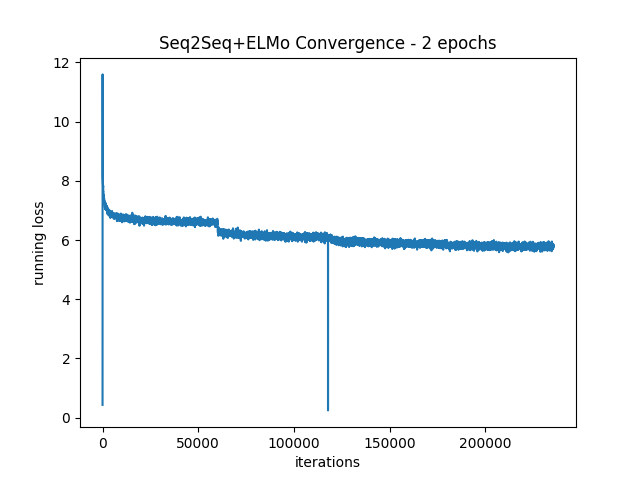
\includegraphics[width=\linewidth]{figures/convergence.png}
\vspace{-8mm}
\caption{\textbf{Learning curve}. The first dip happened around $60,000$ iterations, which is precisely the first time we reduce our learning rate. The two vertical lines are due to numerical instabilities at the beginning of an epoch while calculating the running loss. As one can see, the objective function plateaus after $2$ epochs which suggests the end of training.}
\label{fig: convergence}
\end{figure}

Our model is trained on an NVIDIA GTX 1060 GPU using shuffled minibatches of size $32$. Since we have a large training set, we only ran our model for $2$ epochs and the loss converges in the end (see Fig. \ref{fig: convergence}). Excluding any preprocessing time, training one model takes about $10$ hours, which is the main bottleneck of our study.

We also compare the use of two other word embeddings ($300$-dimension \texttt{GloVe} embeddings, and $300$-dimension \texttt{FastText} embeddings) against \texttt{ELMo} using the same architecture and training procedure. The results are shown in Table \ref{tab: compare_embed}.




